
%%%%%%%%%%%%%%%%%%%%%%%%%%%%%%%%%%%%%%%%%%%%%%%%%%%%%%%%
%
% Copyright (c) 2003-2009 by University of Queensland
% Earth Systems Science Computational Center (ESSCC)
% http://www.uq.edu.au/esscc
%
% Primary Business: Queensland, Australia
% Licensed under the Open Software License version 3.0
% http://www.opensource.org/licenses/osl-3.0.php
%
%%%%%%%%%%%%%%%%%%%%%%%%%%%%%%%%%%%%%%%%%%%%%%%%%%%%%%%%

\section{One Dimensional Heat Diffusion in an Iron Rod}
%\label{Sec:1DHDv0}
We will start by examining a simple one dimensional heat diffusion example. While this exact problem is not strictly relevant to earth sciences; it will provide a good launch pad to build our knowledge of \ESCRIPT and how to solve simple partial differential equations (PDEs) 
\footnote{Wikipedia provides an excellent and comprehensive introduction to \textit{Partial Differential Equations} \url{http://en.wikipedia.org/wiki/Partial_differential_equation}, however their relevance to \ESCRIPT and implementation should become a clearer as we develop our understanding further into the cookbook.}

The first model consists of a simple cold iron bar at a constant temperature of zero Figure \ref{fig:onedhdmodel}. The bar is perfectly insulated on all sides with a heating element of some description at one end. Intuition tells us that as heat is applied; energy will disperse along the bar via convection. With time the bar will reach a constant temperature equivalent to the heat source.
\begin{figure}[h!]
\centerline{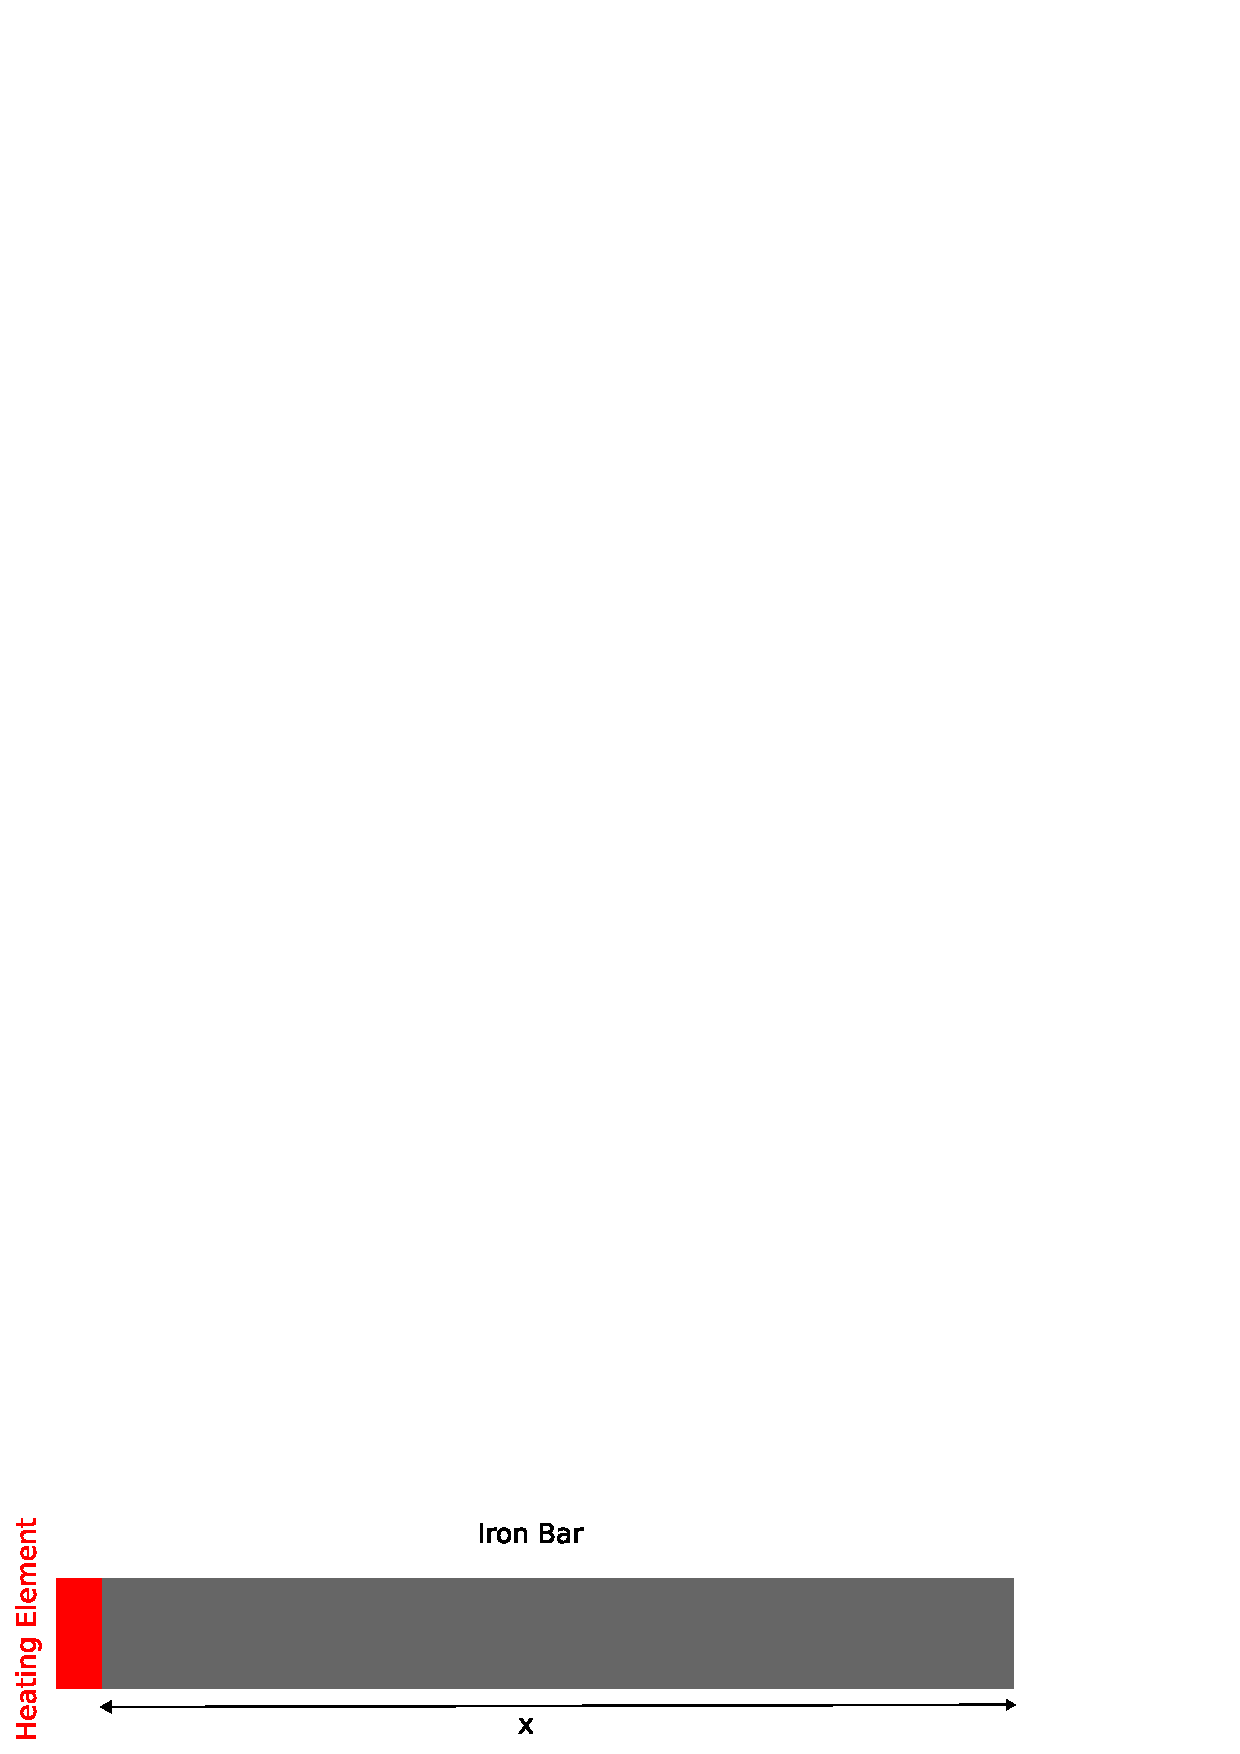
\includegraphics[width=4.in]{figures/onedheatdiff}}
\caption{One dimensional model of an Iron bar.}
\label{fig:onedhdmodel}
\end{figure}

We can model the heat distribution of this problem in time using the one dimensional heat diffusion equation
\footnote{A detailed discussion on how the heat diffusion equation is derived can be found at \url{http://online.redwoods.edu/instruct/darnold/DEProj/sp02/AbeRichards/paper.pdf}};
which is defined as:
\begin{equation}
\rho c\hackscore p \frac{\partial T}{\partial t} - \kappa \frac{\partial^{2} T}{\partial x^{2}} = q\hackscore H 
\label{eqn:hd}
\end{equation}
where $\rho$ is the material density, $c\hackscore p$ is the specific heat and $\kappa$ is the thermal conductivity constant for a given material
\footnote{A list of some common thermal conductivities is available from Wikipedia \url{http://en.wikipedia.org/wiki/List_of_thermal_conductivities}}. 
The heatsource is defined by the right hand side of \eqref{eqn:hd} as $q\hackscore{H}$, this could be a constant or a function of time. For example $q\hackscore{H} = Te^{\gamma t}$ where we have the output of our heatsource decaying with time. There are also two partial derivatives in \eqref{eqn:hd}; $\frac{\partial T}{\partial t}$ describes the change in temperature with time while $\frac{\partial ^2 T}{\partial x^2}$ is the spatial change of temperature. As there is only a single spatial dimension to our problem, our temperature solution $T$ is only dependent on the time $t$ and our position along the iron bar $x$.

When solving a PDE analytically we are finding an exact solution to our equation, however it is not always possible to solve a problem this way. Computers can be used in these cases when a large number of sums or visualisation is required. Computers require a numerical approach to solving problems - \ESCRIPT is one example -  and it becomes necessary to discretize the equation so that we are left with a finite number of equations for a finite number of spatial and time steps in the model. While this is of course an approximation and introduces a degree of error, we find that a sufficiently sampled model is generally accurate enough for the requirements of the modeller.

To solve this equation we will write a simple python script which uses \ESCRIPT and \FINLEY of the \ESYS module. At this point we assume that you have some basic understanding of the python programming language. If not there are some pointers and links available in Section \ref{sec:escpybas} .

In the following section we will develop a script for \ESCRIPT to solve the heat equation step-by-step. Firstly it is necessary to import all the libraries
\footnote{The libraries contain predefined scripts that are required to solve certain problems, these can be simple like sin and cos functions or more complicated like those from our \ESCRIPT library.} 
that we will require.
\begin{verbatim}
from esys.escript import *
from esys.escript.linearPDEs import SingleLinearPDE
from esys.finley import Rectangle
from esys.escript.unitsSI import *
import os
\end{verbatim}
It is generally a good idea to import all of the \verb escript  library, although if you know the packages you need you can specify them individually. The function \verb|LinearPDE| has been imported for ease of use later in the script. \verb|Rectangle| is going to be our type of domain. The package \verb unitsSI  is a module of \esc that provides support for units definitions with our variables; and the \verb|os| package is needed to handle file outputs once our PDE has been solved.

Once our libraries dependancies have been established, defining the problem specific variables is the next step. In general the number of variables needed will vary between problems. These variables belong to two categories. They are either directly related to the PDE and can be used as inputs into the escript solver, or they are script variables used to control internal functions and iterations in our problem. For this PDE there are a number of constants which will need values. Firstly, the domain upon which we wish to solve our problem needs to be defined. There are many different types of domains in escript. We will demonstrate a few in later tutorials but for our iron rod we will simply use a rectangular domain. 

Using a rectangular domain simplifies a \textit{3D} object into a single dimension. The iron rod will have a lengthways cross section that looks like a rectangle.  As a result we do not need to model the volume of the rod because a cylinder is symmetrical about its center. There are four arguments we must consider when we decide to create a rectangular domain, the model length, width and step size in each direction. When defining the size of our problem it will help us determine appropriate values for our domain arguments. If we make our dimensions large but our step sizes very small we will to a point, increase the accuracy of our solution. Unfortunately we also increase the number of calculations that must be solved per time step. This means more computational time is required to produce a solution. In our \textit{1D} problem we will define our bar as being 1 metre long. An appropriate \verb|ndx| would be 1 to 10\% of the length. Our \verb|ndy| need only be 1, This is because our problem stipulates no partial derivatives in the $y$ direction so the temperature does not vary with $y$. Thus the domain perameters can be defined as follows; note we have used the \verb unitsSI  convention to make sure all our input units are converted to SI.
\begin{verbatim}
#Domain related.
mx = 1*m #meters - model lenght
my = .1*m #meters - model width
ndx = 100 # steps in x direction 
ndy = 1 # steps in y direction
\end{verbatim}
The material constants and the temperature variables must also be defined. For the iron rod in the model they are defined as:
\begin{verbatim}
#PDE related
q=200. * Celsius #Kelvin - our heat source temperature
Tref = 0. * Celsius # Kelvin - starting temp of iron bar
rho = 7874. *kg/m**3 #kg/m^{3} density of iron
cp = 449.*J/(kg*K) #jules/Kg.K thermal capacity
rhocp = rho*cp
kappa = 80.*W/m/K #watts/m.K thermal conductivity
\end{verbatim}
Finally, to control our script we will have to specify our timing controls and where we would like to save the output from the solver. This is simple enough:
\begin{verbatim}
#Script/Iteration Related
t=0 #our start time, usually zero
tend=5.*60. #seconds - time to end simulation
outputs = 200 # number of time steps required.
h=(tend-t)/outputs #size of time step
i=0 #loop counter 
#the folder to put our outputs in, leave blank "" for script path
#note this folder path must exist to work
save_path = "data/onedheatdiff001" 
\end{verbatim}
Now that we know our inputs we will build a domain using the \verb Rectangle() function from \verb Finley . The four arguments allow us to define our domain \verb rod  as:
\begin{verbatim}
 rod = Rectangle(l0=mx,l1=my,n0=ndx,n1=ndy)
\end{verbatim}
In this form \verb rod does not represent any discrete points, but rather an area of \verb ndx*ndy  cells that fit into a rectangular space with opposing vertices at the origin and the point \verb [mx,my] . Our domain is contructed this way to allow the user to determine where the discrete points of each model will be located. Discretisation may be at the corners of each cell, the middle point of a cell or halfway along each side of the cell etc. Depending on the PDE or the model there may be advantages and disadvantages for each case. Fortunately \verb escript offers an easy way to extract finite points from the domain \verb|rod| using the domain property function \verb|getX()| . This function sets the vertices of each cell as finite points to solve in the solution. If we let \verb|x| be these finite points, then;
\begin{verbatim}
 x = rod.getX()
\end{verbatim}
With a domain and all our required variables established, it is now possible to set up our PDE so that it can be solved by escript. The first step is to define the type of PDE that we are trying to solve in each time step. In this example it is a single linear PDE
\footnote{in comparison to a system of PDEs which will be discussed later.}
we can define by:
\begin{verbatim}
 mypde=LinearSinglePDE(rod)
\end{verbatim}
In the next step we need to define the coefficients of the PDE. The linear
PDEs in \ESCRIPT provide a general interface to do this. Here we will only discuss a simplified form that suits our heat diffusion problem and refer to the \ESCRIPT user's guide for the general case. This simpler form
\footnote{In the form of the \ESCRIPT users guide which using the Einstein convention is written as 
$-(A\hackscore{jl} u\hackscore{,l})\hackscore{,j}+D u =Y$}
is described by;
\begin{equation}\label{eqn:commonform nabla}
-\nabla.(A.\nabla u) + Du = f
\end{equation}
where $A$, $D$ and $f$ are known values. The symbol $\nabla$ which is called the \textit{Nabla operator} or \textit{del operator} represents
the spatial derivative of its subject - in this case $u$. Lets assume for a moment that we deal with a one-dimensional problem then 
\begin{equation}
\nabla = \frac{\partial}{\partial x}
\end{equation}
and we can write equation \ref{eqn:commonform nabla} as
\begin{equation}\label{eqn:commonform}
-A\frac{\partial^{2}u}{\partial x^{2}} + Du = f
\end{equation}
if $A$ is constant then equation \ref{eqn:commonform} is consistent with our heat diffusion problem in Equation \ref{eqn:hd} - except for $u$. When comparing equations \eqref{eqn:hd} and \eqref{eqn:commonform} we see that;
\begin{equation}
A = \kappa; D = \rho c \hackscore{p}; f = q \hackscore{H}
\end{equation}

We can write the partial $\frac{\partial T}{\partial t}$ in terms of $u$ by discretising the time of our solution. Many methods could be used here but we have decided on the Backwards Euler approximation which states;
\begin{equation}
f'(x) \approx \frac{f(x+h)-f(x)}{h}
\label{eqn:beuler}
\end{equation}
where h is the the discrete step size $\Delta x$.
Now let $f(x) = T(t)$ and from equation \ref{eqn:beuler} we see that;
\begin{equation}
T'(t) \approx \frac{T(t+h) - T(t)}{h}
\end{equation}
which can also be written as;
\begin{equation}
T\hackscore{,t}^{(n)} \approx \frac{T^{(n)} - T^{(n-1)}}{h}
\label{eqn:Tbeuler}
\end{equation}
where $n$ denotes the n\textsuperscript{th} time step. Substituting equation \ref{eqn:Tbeuler} into equation \ref{eqn:hd} we get;
\begin{equation}
\frac{\rho c\hackscore p}{h} (T^{(n)} - T^{(n-1)}) - \kappa \frac{\partial^{2} T}{\partial x^{2}} = q\hackscore H 
\label{eqn:hddisc}
\end{equation}
To fit our simplified general form we can rearrange so that;
\begin{equation}
\frac{\rho c\hackscore p}{h} T^{(n)} - (\kappa T^{(n)}\hackscore{,i})\hackscore{,i} = q\hackscore H +  \frac{\rho c\hackscore p}{h} T^{(n-1)}
\label{eqn:hdgenf}
\end{equation}
This is the form required for escript to solve our PDE across the domain for successive time nodes $t^{(n)}$ where 
$t^{(0)}=0$ and  $t^{(n)}=t^{(n-1)}+h$ where $h>0$ is the step size which is assumed to be constant. 
In the following the upper index ${(n)}$ refers to a value at time $t^{(n)}$. When comparing equation \ref{eqn:hdgenf} with equation \ref{eqn:commonform} we see that;
\begin{equation}
A = \kappa; D = \frac{\rho c \hackscore{p}}{h}; f = q \hackscore{H} + \frac{\rho c\hackscore p}{h} T^{(n-1)}
\end{equation}

\TODO{DISCUSS BOUNDARY CONDITIONS}
It is pointed out that the initial conditions satisfy the boundary condition defined by 

Together with the natural boundary condition 
\begin{equation}
 \kappa T\hackscore{,i}^{(n)} n\hackscore i = \eta (T\hackscore{ref}-T^{(n)}) 
\label{DIFFUSION TEMP EQ 2222}
\end{equation}
taken from 
this forms a boundary value problem that has to be solved for each time step. 
As a first step to implement a solver for the temperature diffusion problem we will 
first implement a solver for the  boundary value problem that has to be solved at each time step.

We need to revisit the general PDE equation ~\ref{eqn:commonform nabla} under the light of a two dimensional domain. \ESCRIPT is inherently designed to solve problems that are greater than one dimension and so \ref{eqn:commonform nabla} needs to be read as a higher dimensional problem. In the case of two spatial dimensions the Nabla operator has in fact two components $\nabla = (\frac{\partial}{\partial x}, \frac{\partial}{\partial y})$. In full the general equation ~\ref{eqn:commonform nabla} assuming a constant coefficient $A$ takes the form;
\begin{equation}\label{eqn:commonform2D}
-A\hackscore{00}\frac{\partial^{2}u}{\partial x^{2}} 
-A\hackscore{01}\frac{\partial^{2}u}{\partial x\partial y} 
-A\hackscore{10}\frac{\partial^{2}u}{\partial y\partial x} 
-A\hackscore{11}\frac{\partial^{2}u}{\partial y^{2}} 
+ Du = f
\end{equation}
We notice that for the higher dimensional case $A$ becomes a matrix. It is also
important to notice that the usage of the Nable operator creates
a compact formulation which is also independant from the spatial dimension. 
So to make the general PDE~\ref{eqn:commonform2D} one dimensional as
shown in~\ref{eqn:commonform} we need to set
\begin{equation}\label{eqn:commonform2D}
A\hackscore{00}=A; A\hackscore{01}=A\hackscore{10}=A\hackscore{11}=0
\end{equation}

Now that we have established the general form we will submit to escript it is necessary to establish the state of our system at time zero or $T^{(n=0)}$. This is due to the time derivative approximation we have used. We have chosen the starting temperature of our iron bar to be 0$\deg C$ . The temperature becomes;
\begin{equation}
T(x,0) = T\hackscore{ref} = 0
\end{equation}
for all $x$ in the domain. 

Because we have a symmetrical problem we will also need to set the symmetry on by:
\begin{verbatim}
 myPDE.setSymmetryOn()
\end{verbatim}

Additionally we must also consider the boundary conditions of our PDE. They take the form:
\begin{equation}
\eta \hackscore{j} A\hackscore{jl} u\hackscore{,l} + du = y
\end{equation}


NEED TO WORK ON THIS SECTION

We now need to specify Our boundary conditions and initial values. The initial values required to solve this PDE are temperatures for each discrete point in our domain that we wish to solve for. We will set our bar to:
\begin{verbatim}
 T = Tref
\end{verbatim}
Boundary conditions are a little more difficult. Fortunately the escript solver will handle our insulated boundary conditions. However, we will need to apply our heat source $q_{H}$ to the end of the bar at $x=0$ . escript makes this easy by letting us define areas in our domain. To retrieve all the finite points in our domain we will use 

END WORK ON THIS SECTION

\section{Plot total heat} 
\TODO{show the script}

\TODO{explain how to use matlibplot to visualize the total heat integral(rho*c*T) over time}

\section{Plot Temperature Distribution}
\TODO{explain how to use matlibplot to visualize T}

 
